\documentclass{beamer}
\usepackage{../common_slides}
\usepackage{pdfpages}
\usepackage{stackengine}
\stackMath
\newlength\matfield
\newlength\tmplength
\def\matscale{1.}
\newcommand\dimbox[3]{%
  \setlength\matfield{\matscale\baselineskip}%
  \setbox0=\hbox{\vphantom{X}\smash{#3}}%
  \setlength{\tmplength}{#1\matfield-\ht0-\dp0}%
  \fboxrule=1pt\fboxsep=-\fboxrule\relax%
  \fbox{\makebox[#2\matfield]{\addstackgap[.5\tmplength]{\box0}}}%
}
\newcommand\raiserows[2]{%
   \setlength\matfield{\matscale\baselineskip}%
   \raisebox{#1\matfield}{#2}%
}
\newcommand\matbox[4]{
  \stackunder{\dimbox{#1}{#2}{$#4$}}{\scriptstyle #3}%
}

\title{Part-of-Speech Tagging \\ + \\ Neural Networks 2}
\date{}
\author{CS 287}
\begin{document}
\maketitle{}

\begin{frame}{Review:  Bilinear Model}
  Bilinear model,
  \[\hat{\boldy} = (\boldx^0 \boldW^0)\boldW^1 + \boldb)\]
  \begin{itemize}
  \item $\boldx^0 \in \reals^{1 \times d_0}$ start with one-hot.
  \item $\boldW^0 \in \reals^{d_0 \times \din}$, $d_0 = |\mcF|$
  \item $\boldW^1 \in \reals^{\din \times \dout}, \boldb \in \reals^{1 \times \dout}$; model parameters
  \end{itemize}
  \air
  Notes:
  \begin{itemize}
  \item Bilinear parameter interaction.
  \item $d_0 >> \din$, e.g. $d_0 = 10000, \din = 50$
  \end{itemize}

\end{frame}

\begin{frame}{Review:  Bilinear Model: Intuition}
  \[ (\boldx^0 \boldW^0)\boldW^1 + \boldb\]


  \[
    \begin{bmatrix}
      0 & \ldots & \textcolor{red}{1} & \ldots & 0 \\
    \end{bmatrix}
    \begin{bmatrix}
      w^0_{1,1} &  \ldots &w^0_{0, \din}\\
      & \vdots & \\
      & \vdots & \\
      & \vdots & \\
      \textcolor{red}{w^0_{k,1}} &  \textcolor{red}{\ldots} &\textcolor{red}{w^0_{k,\din}}\\
      & \vdots & \\
      & \vdots & \\
      & \vdots & \\
      w^0_{d_0, 1} &  \ldots &w^0_{d_0, \din}\\
    \end{bmatrix}
    \begin{bmatrix}
      \textcolor{red}{w^1_{1,1}} &  \ldots & \ldots &   \textcolor{red}{w^1_{0, \dout}}\\
      & \ddots & \ddots &  \\
      \textcolor{red}{w^1_{\din,0}} &  \ldots & \ldots & \textcolor{red}{w^1_{\din, \dout}}\\
    \end{bmatrix}
  \]

\end{frame}

\begin{frame}{Review:  Window Model}
  \textbf{Goal:} predict $t_5$.


  \begin{itemize}
  \item Windowed word model.

  \[ w_1\ w_2\ [\textcolor{red}{w_3\ w_4\ w_5\ w_6\ w_7}]\ w_8 \]

  \item $w_3, w_4$; left context
  \item $w_5$; Word of interest
  \item $w_6, w_7$; right context

  \item $\dwin$; size of window ($\dwin = 5$)
  \end{itemize}
\end{frame}

\begin{frame}{Review: Dense Windowed BoW Features }
  \begin{itemize}
  \item $f_1, \ldots, f_{\dwin}$ are words in window
  \item Input representation is the concatenation of embeddings
  \end{itemize}

  \[ \boldx = [v(f_1)\  v(f_2) \  \ldots \  v(f_{\dwin})]  \]

  Example: Tagging
  \[ w_1\ w_2\ [\textcolor{red}{w_3\ w_4\ w_5\ w_6\ w_7}]\ w_8 \]
  \[ \boldx = [v(w_3)\  v(w_4) \  v(w_5) \ v(w_6) \ v(w_7)]  \]

  \[\renewcommand\matscale{.6}
\matbox{1.5}{4}{\din /5}{} \matbox{1.5}{4}{\din /5}{} \matbox{1.5}{4}{\din /5}{\boldx} \matbox{1.5}{4}{\din /5}{} \matbox{1.5}{4}{\din /5}{}% \raiserows{1.5}{\matbox{4}{2}{d_0}{\dout}{\boldW^0}}  \matbox{4}{2}{\din}{\dout}{\boldW^1} +
% \matbox{7}{2}{1}{\dout}{\boldb}
\]

Rows of $\boldW^1$ encode position specific weights.
\end{frame}


\begin{frame}{Quiz}
  We are doing tagging with a windowed bilinear model with hinge-loss
  and no capitalization features. The model has $\dwin = 5$,
  $\din = 50$, $\dout = 40$, and vocabulary size $10000$.

  \air

  We are given the input window:

  \air


  \begin{center}
    \texttt{The dog walked to the}
  \end{center}

  Unfortunately we incorrectly classify \texttt{walked} as \texttt{NN}
  as opposed to \texttt{VP}, in a bilinear model with a hinge-loss .
  \air


  What is the maximum number of parameters that
  receive a non-zero gradient?
\end{frame}


\begin{frame}{Answer: }
  \begin{center}






  \[{\tiny
    \begin{bmatrix}
       \textcolor{red}{1}   & \textcolor{red}{1} &  \textcolor{red}{1} &
 \textcolor{red}{1}  & \textcolor{red}{1} \\
    \end{bmatrix}
    \begin{bmatrix}
      w^0_{1,1} &  \ldots &w^0_{0, \din}\\
      \textcolor{red}{w^0_{the,1}} &  \textcolor{red}{\ldots} &\textcolor{red}{w^0_{the,\din}}\\
      \vdots \\
      \textcolor{red}{w^0_{dog,1}} &  \textcolor{red}{\ldots} &\textcolor{red}{w^0_{dog,\din}}\\
      \vdots \\
      \textcolor{red}{w^0_{walked,1}} &  \textcolor{red}{\ldots} &\textcolor{red}{w^0_{walked,\din}}\\
      \vdots \\
      \textcolor{red}{w^0_{to,1}} &  \textcolor{red}{\ldots} &\textcolor{red}{w^0_{to,\din}}\\
      \vdots \\
      \textcolor{red}{w^0_{the,1}} &  \textcolor{red}{\ldots} &\textcolor{red}{w^0_{the,\din}}\\
      \vdots \\
      w^0_{d_0, 1} &  \ldots &w^0_{d_0, \din}\\
    \end{bmatrix}
    \begin{bmatrix}
      w^1_{1,1} &  \ldots&  \textcolor{red}{w^1_{1,NN}} & \ldots &  \textcolor{red}{w^1_{1,VP}} &    w^1_{0, \dout}\\
                & \ddots & \ddots &                    &         &                                   &  \\
      w^1_{\din,0} &  \ldots&  \textcolor{red}{w^1_{\din,NN}} & \ldots &  \textcolor{red}{w^1_{\din,VP}} &  w^1_{\din, \dout}\\
    \end{bmatrix}
    }
  \]



\air

  $\boldW^0 = 5 \times \din$

  $\boldW^1 = \din \times 2$
  \end{center}

\end{frame}


\begin{frame}{Part-of-Speech Tagging 1}
  Consider the following windowed model, and
  assume for now a linear model.

  \[ [ w_1\ \mathrm{\texttt{the}}\ w_3\ w_4\ w_5 ]\]


  \begin{itemize}
  \item What information do we have about the tag of $w_3$?
    \air

  \item What weight should the features values associated with
    \texttt{the} in position $w_2$ take?
  \end{itemize}
\end{frame}

\begin{frame}{Part-of-Speech Tagging 2}
  Next Consider the following windowed model, and
  assume for now a linear model.

  \[[ w_1\ w_2 \ w_3\ \mathrm{\texttt{dog}} \ w_5 ]\]


  \begin{itemize}
  \item What information do we have about the tag of $w_3$?
    \air

  \item What weight should the features values associated with
    \texttt{dog} in position $w_4$ take?
  \end{itemize}

\end{frame}


\begin{frame}{Part-of-Speech Tagging 3}
  Now finally consider the following windowed model, and
  assume for now a linear model.

  \[[w_1\ \texttt{the} \ w_3\ \mathrm{\texttt{dog}} \ w_5] \]


  \begin{itemize}
  \item What information do we have about the tag of $w_3$?
    \air

  \item What weight would we want if we combined both the features values?
  \end{itemize}

\end{frame}

\section{Neural Networks}

\begin{frame}
  \begin{center}
    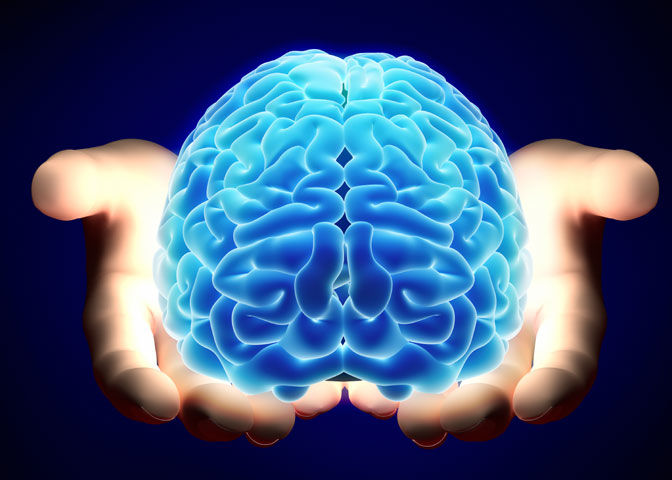
\includegraphics[width=5cm]{brain}
  \end{center}
\end{frame}

\begin{frame}{Neural Network}
  One-layer multi-layer perceptron architecture,

  \[NN_{MLP1}(\boldx) =  g(\boldx\boldW^1 + \boldb^1)W^2 + \boldb^2\]
  \begin{itemize}
  \item $\boldx\boldW + \boldb$; \textit{perceptron}
  \item $\boldx$ is the dense representation in $\reals^{1 \times \din}$
  \item $\boldW^1 \in \reals^{\din \times \dhid}, \boldb^1 \in \reals^{1 \times \dhid}$; first affine transformation
  \item $\boldW^2 \in \reals^{\dhid \times \dout}, \boldb^2 \in \reals^{1 \times \dout}$; second affine transformation
  \item $g:\reals^{\dhid \times \dhid}$ is an \textit{activation non-linearity} (often pointwise)
  \item $g(\boldx\boldW^1 + \boldb^1)$ is the \textit{hidden layer}
  \end{itemize}
\end{frame}

\begin{frame}{Schematic}
  \begin{center}


  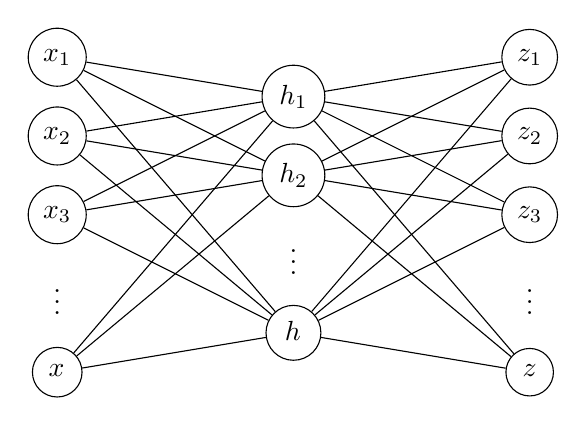
\begin{tikzpicture}
    \node(aa)[draw, circle]{$x_1$};
    \node(ab)[below of =  aa, draw, circle]{$x_2$};
    \node(ac)[below of = ab, draw,circle]{$x_3$};
    \node(ad)[below of = ac]{$\vdots$};
    \node(ae)[below of =  ad, draw, circle]{$x_{\din}$};


    \node(ba)[xshift= 2cm, yshift=-0.5cm, right of = aa, draw, circle]{$h_1$};
    \node(bb)[below of =  ba, draw, circle]{$h_2$};
    \node(bc)[below of = bb]{$\vdots$};

    \node(bd)[below of =  bc, draw, circle]{$h_{\dhid}$};

    \path[draw] (aa) -- (ba);
    \path[draw] (aa) -- (bb);
    \path[draw] (aa) -- (bd);

    \path[draw] (ab) -- (ba);
    \path[draw] (ab) -- (bb);
    \path[draw] (ab) -- (bd);

    \path[draw] (ac) -- (ba);
    \path[draw] (ac) -- (bb);
    \path[draw] (ac) -- (bd);

    \path[draw] (ae) -- (ba);
    \path[draw] (ae) -- (bb);
    \path[draw] (ae) -- (bd);


    \node(ca)[xshift= 2cm, yshift=0.5cm, right of = ba, draw, circle]{$z_1$};
    \node(cb)[below of =  ca, draw, circle]{$z_2$};
    \node(cc)[below of =  cb, draw, circle]{$z_3$};
    \node(cd)[below of = cc]{$\vdots$};
    \node(ce)[below of =  cd, draw, circle]{$z_{\dout}$};


    \path[draw] (ba) -- (ca);
    \path[draw] (ba) -- (cb);
    \path[draw] (ba) -- (cc);
    \path[draw] (ba) -- (ce);

    \path[draw] (bb) -- (ca);
    \path[draw] (bb) -- (cb);
    \path[draw] (bb) -- (cc);
    \path[draw] (bb) -- (ce);

    \path[draw] (bd) -- (ca);
    \path[draw] (bd) -- (cb);
    \path[draw] (bd) -- (cc);
    \path[draw] (bd) -- (ce);


  \end{tikzpicture}
  \end{center}
\end{frame}


\begin{frame}{Non-Linearities: 0/1}
  0/1 function:
  \[0/1(t) = \indicator(t > 0) \]
  \begin{figure}
    \centering
    \includegraphics[width=5cm]{../notebooks/01}
  \end{figure}

  \begin{itemize}
  \item $01((\boldx\boldW^1 + \boldb^1)_i)$
  \item Intuition: On, if above a threshold
  \end{itemize}
\end{frame}


\begin{frame}{Exercise}
  Input layer to $NN_{MLP1}$ is the sparse indicator features
  of the word at each position.

  \begin{itemize}
  \item Design a network to recognize
  \[[w_1\ \texttt{the} \ w_3\ \mathrm{\texttt{dog}} \ w_5] \]

  \item Design a network to recognize  where $w_2$ is not \texttt{the}
  \[[w_1\ w_2 \ w_3\ \mathrm{\texttt{dog}} \ w_5] \]

  \end{itemize}
\end{frame}

\begin{frame}{Feature Conjunctions}
  Many NLP tasks require conjunctive features, examples
  \begin{itemize}
  \item Sequence-based taggers look at last two-part of speech tags.
    \air

  \item Chinese part-of-speech taggers look at first character and last tag.
    \air

  \item Higher-level models (parses) look at tags of words and distances apart (example)
  \end{itemize}
  \air

  For some natural language tasks, conjunctions are painstakingly hard.

  \pause
  \begin{itemize}
  \item NNs: Capacity to learn conjunctions and feature combinations.
    \air

  \item Also possible with other convex models such as SVMs
  \end{itemize}
\end{frame}

{
\setbeamercolor{background canvas}{bg=}
\includepdf[pages=14]{swacl15}
\includepdf[pages=16]{swacl15}
}


\begin{frame}{Non-Linearities: 0/1}
  0/1 function:
  \[0/1(t) = \indicator(t > 0) \]
  \begin{figure}
    \centering
    \includegraphics[width=5cm]{../notebooks/01}
    \includegraphics[width=5cm]{../notebooks/01grad}
  \end{figure}

  \begin{itemize}
  \item Issue: No gradient anywhere
  \end{itemize}
\end{frame}

\begin{frame}{Non-Linear Functions: Sigmoid}
  Logistic sigmoid function:
  \[\sigma(t) = \frac{1}{1 + \exp(-t)} \]
  \begin{figure}
    \centering
    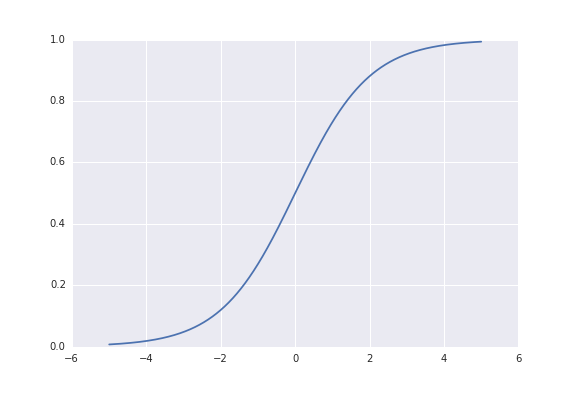
\includegraphics[width=5cm]{../notebooks/sigmoid}     \includegraphics[width=5cm]{../notebooks/sigmoidgrad}
  \end{figure}

  \begin{itemize}
  \item $\sigma((\boldx\boldW^1 + \boldb^1)_i)$
  \item Intuition: Each hidden dimension (``neuron'') is result of logistic regression.
  \end{itemize}
\end{frame}


\begin{frame}{Other Non-Linearities: ReLU}
  Rectified Linear Unit:
  \begin{figure}
    \centering
    \[\relu(t) = \max\{0, t\} \]
    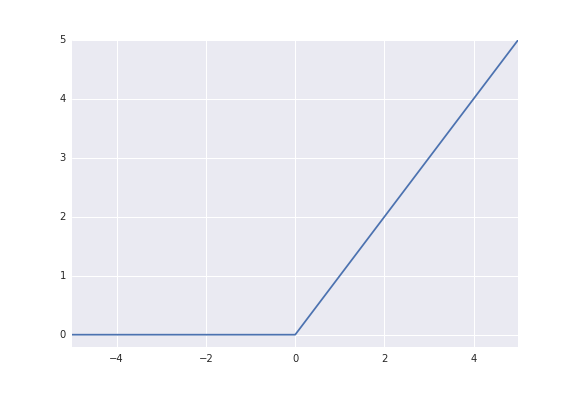
\includegraphics[width=5cm]{../notebooks/Relu}
    \includegraphics[width=5cm]{../notebooks/Relugrad}
  \end{figure}
  \begin{itemize}
  \item Intuition: Each hidden-unit gives activation margin
  \item No gradient (saturation) when below 0.
  \end{itemize}
\end{frame}

\begin{frame}{Saturation: Intuition}
  \begin{center}
  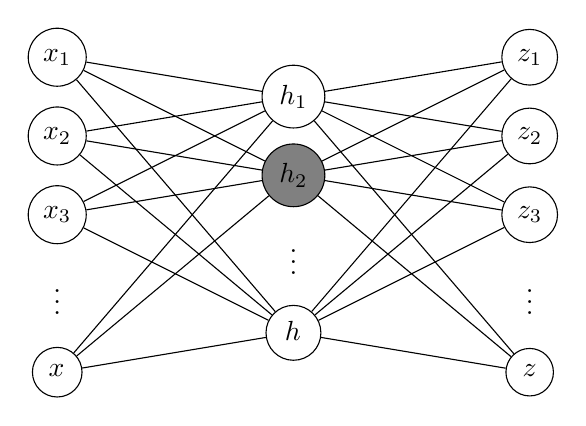
\begin{tikzpicture}
    \node(aa)[draw, circle]{$x_1$};
    \node(ab)[below of =  aa, draw, circle]{$x_2$};
    \node(ac)[below of = ab, draw,circle]{$x_3$};
    \node(ad)[below of = ac]{$\vdots$};
    \node(ae)[below of =  ad, draw, circle]{$x_{\din}$};


    \node(ba)[xshift= 2cm, yshift=-0.5cm, right of = aa, draw, circle]{$h_1$};
    \node(bb)[below of =  ba, draw, fill=gray, circle]{$h_2$};
    \node(bc)[below of = bb]{$\vdots$};

    \node(bd)[below of =  bc, draw, circle]{$h_{\dhid}$};

    \path[draw] (aa) -- (ba);
    \path[draw] (aa) -- (bb);
    \path[draw] (aa) -- (bd);

    \path[draw] (ab) -- (ba);
    \path[draw] (ab) -- (bb);
    \path[draw] (ab) -- (bd);

    \path[draw] (ac) -- (ba);
    \path[draw] (ac) -- (bb);
    \path[draw] (ac) -- (bd);

    \path[draw] (ae) -- (ba);
    \path[draw] (ae) -- (bb);
    \path[draw] (ae) -- (bd);


    \node(ca)[xshift= 2cm, yshift=0.5cm, right of = ba, draw, circle]{$z_1$};
    \node(cb)[below of =  ca, draw, circle]{$z_2$};
    \node(cc)[below of =  cb, draw, circle]{$z_3$};
    \node(cd)[below of = cc]{$\vdots$};
    \node(ce)[below of =  cd, draw, circle]{$z_{\dout}$};


    \path[draw] (ba) -- (ca);
    \path[draw] (ba) -- (cb);
    \path[draw] (ba) -- (cc);
    \path[draw] (ba) -- (ce);

    \path[draw] (bb) -- (ca);
    \path[draw] (bb) -- (cb);
    \path[draw] (bb) -- (cc);
    \path[draw] (bb) -- (ce);

    \path[draw] (bd) -- (ca);
    \path[draw] (bd) -- (cb);
    \path[draw] (bd) -- (cc);
    \path[draw] (bd) -- (ce);
  \end{tikzpicture}
  \end{center}
\end{frame}


\begin{frame}{Other Non-Linearities: Tanh}
  Hyperbolic Tangeant:
  \begin{figure}
    \centering
    \[\tanh(t) = \frac{\exp(t) - \exp(-t)}{\exp(t) + \exp(-t)}  \]
    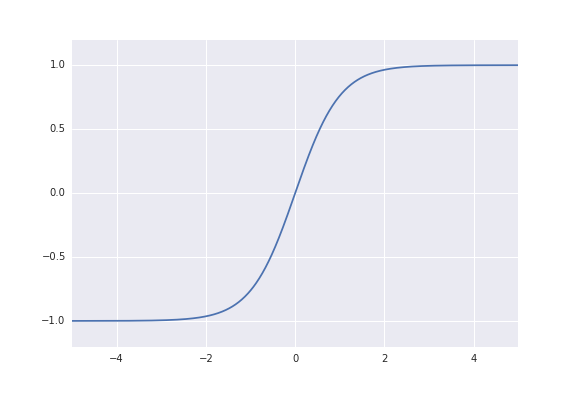
\includegraphics[width=5cm]{../notebooks/tanh}
    \includegraphics[width=5cm]{../notebooks/tanhgrad}
  \end{figure}
  \begin{itemize}
  \item Intuition: Similar to sigmoid, but range between 1 and -1.
  \end{itemize}
\end{frame}


\begin{frame}{Other Non-Linearities: Hard Tanh}
  Hyperbolic Tangeant:
  \begin{figure}
    \centering
    \[\mathrm{hardtanh}(t) =
      \begin{cases}
        -1& t < -1 \\
        t & -1
\leq t \leq 1\\
        1 & t > 1\\
      \end{cases}
    \]
    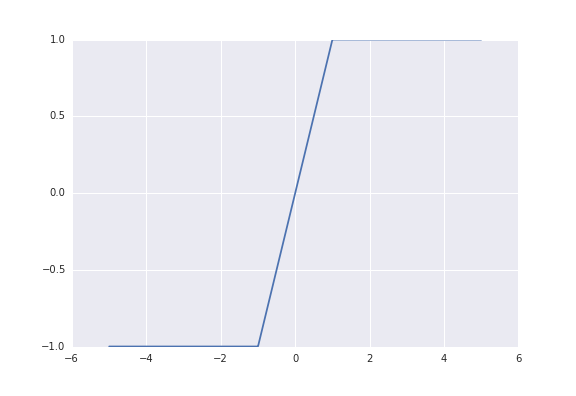
\includegraphics[width=5cm]{../notebooks/hardtanh}
    \includegraphics[width=5cm]{../notebooks/hardtanhgrad}
  \end{figure}
  \begin{itemize}
  \item Intuition: Similar to sigmoid, but range between 1 and -1.
  \end{itemize}
\end{frame}


\begin{frame}{Other Non-Linearities: Cube}
  Cube non-linearity (directly encourage parameter interaction):
  \begin{figure}
    \centering
    \[\mathrm{cube}(t) = t^3  \]
    \includegraphics[width=5cm]{../notebooks/cube}
    \includegraphics[width=5cm]{../notebooks/cubegrad}
  \end{figure}
  \begin{itemize}
  \item Intuition: Directly encourage higher-order interactions.
  \end{itemize}
\end{frame}


\begin{frame}{Tagging from Scratch}
  \begin{center}
    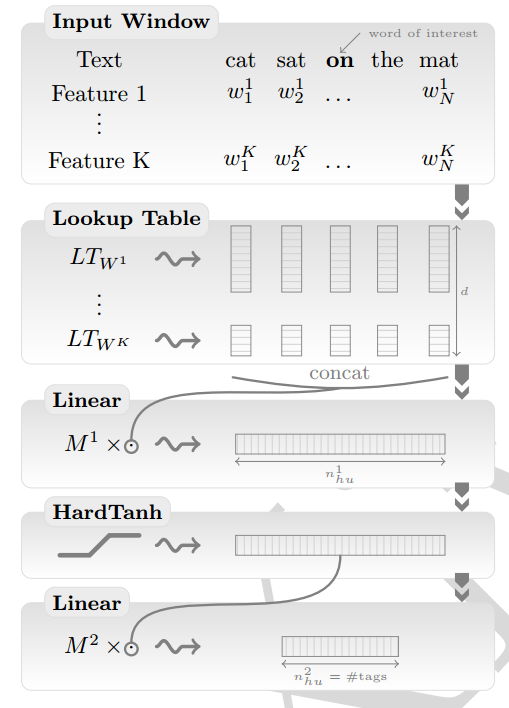
\includegraphics[width=5cm]{cwfull}
  \end{center}
\end{frame}



\begin{frame}{Function Approximator}
  MLP1 is a universal approximator

  \begin{quote}
    Can approximate with any desired non-zero amount of error a family
    of functions that include all continuous functions on a closed and
    bounded subset of $\reals^n$, and any function mapping from any
    finite dimensional discrete space to another (YG)
  \end{quote}

  Caveats:
  \begin{itemize}
    \item Does not give size of hidden layer.
    \item Does not specify how hard this is to learn.
  \end{itemize}
\end{frame}

\begin{frame}{Deep Neural Networks (DNNs)}

  Can stack MLPs, create deep fully connected networks,

  \[NN_{MLP1}(\boldx) =  g(\boldx\boldW^1 + \boldb^1)W^2 + \boldb^2\]
  \[NN_{MLP2}(\boldx) =  g(NN_{MLP1}(\boldx) \boldW^1 + \boldb^1)W^2 + \boldb^2\]

  \begin{itemize}
  \item Can have multiple hidden layers, etc.
  \item Benefit: may be able to find better function
  \item Known to be harder to train (although other approaches)
  \end{itemize}
\end{frame}


\begin{frame}{Other Layers}
  We will discuss many other neural network layers,
  \begin{itemize}
  \item convolutional
  \item attention-based
  \item gated layers
  \item $\ldots$
  \end{itemize}
\end{frame}

{
\setbeamercolor{background canvas}{bg=}


\includepdf[pages=41-42]{highway}
}




\section{Backpropagation}

\begin{frame}{Sequential Neural Network}
  Sequential neural networks consist of a series of composed functions,

  Consider a vector-valued parameterized functions $f_1, \ldots, f_{k}$ where

  \begin{itemize}
  \item $f_i(\boldx;\btheta_i): \reals^{n_{i-1}} \mapsto \reals^{n_{i}}$; function
  \item $\btheta \in \reals^{d_i}$; function parameters
  \end{itemize}

  Consider a scalar-valued loss function  $L(\boldy, \hat{\boldy})$ where

  \begin{itemize}
  \item $L(\boldy, *): \reals^{n_k} \mapsto \reals$; loss for input
  \end{itemize}
\end{frame}


\begin{frame}{Backpropagation}
  \begin{itemize}
  \item Forward Step (f-prop):

    Compute \[L(f_k(\ldots f_1(\boldx^0)))\]
    Saving intermediary values
    \[f_i(\ldots f_1(\boldx^0)))\]
  \item Backward Step (b-prop):
    \pause
    \[ \frac{\partial L}{\partial f_i(\ldots f_1(\boldx^0))  } = \sum_{j =1}^{n_i} \frac{\partial f_{i+1}(\ldots f_1(\boldx^0))_j} {\partial f_i(\ldots f_1(\boldx^0)) } \frac{\partial L} {\partial f_{i+1}(\ldots f_1(\boldx^0))}_j   \]
    \pause

    \[ \frac{\partial L}{\partial \btheta_i  } = \sum_{j =1}^{n_i} \frac{\partial f_{i+1}(\ldots f_1(\boldx^0))_j} {\partial \btheta_i } \frac{\partial L} {\partial f_{i+1}(\ldots f_1(\boldx^0))}_j   \]

  \end{itemize}
\end{frame}

\begin{frame}{Backpropagation: Data flow}
  \begin{center}

  \begin{tikzpicture}
    \node(x){$f_{i}(\ldots f_{1}(\boldx^0)) $};
    \node(t)[below right= of x, draw]{$f_{i+1}(*;\btheta_{i+1})$};

    \node(fx)[above right=of t]{$f_{i+1}(f_{i}(\ldots f_{1}(\boldx^0)))$};
    \node(gradin)[below left =of t]{$\displaystyle \frac{\partial L}{\partial f_i(\ldots f_1(\boldx^0))  } $};
    \node(gradout)[below right= of t]{$\displaystyle  \frac{\partial L}{\partial f_{i+1}(\ldots f_1(\boldx^0))  }  $};
    \node(gradweight)[below = of t, yshift=1cm]{$\displaystyle  \frac{\partial L}{\partial \btheta_{i+1}  }$};
    \path[draw, ->] (x) -> (t);
    \path[draw, ->] (t) -> (fx);
    \path[draw, ->] (t) -> (gradin);
    \path[draw, ->]  (gradout) -> (t);
  \end{tikzpicture}
  \end{center}
\end{frame}

\begin{frame}{Torch Implementation}
  Torch uses declarative unit-based specification of NN
  \begin{itemize}
  \item Every function is a represented as a unit.
    \air

  \item Responsibilities:
    \begin{enumerate}
    \item Expose any parameters $\btheta_{i+1}$ as tensors
    \item Compute $f_{i+1}(\boldx, \btheta_{i+1})$ (fprop)
    \item Compute any necessary state needed for bprop
    \item Compute chain-rule given  $\frac{\partial L}{\partial f_{i+1}(\ldots f_1(\boldx^0))}$ and $f_{i}(\ldots f_1(\boldx^0))$
    \item Compute parameter gradient $\frac{\partial L}{\partial \btheta_{i+1}} $
    \end{enumerate}
  \item Contract: forward will always be called before backward.
  \end{itemize}
\end{frame}

\begin{frame}{Torch Units}
  \begin{center}

  \begin{tikzpicture}
    \node(x)[text width=3cm,text centered]{input\\ $f_{i}(\ldots f_{1}(\boldx^0)) $};
    \node(t)[text  width=3cm,text centered, below right= of x, draw]{weights \\ $f_{i+1}(*;\btheta_{i+1})$};

    \node(fx)[text width=3cm,text centered, above right=of t]{self.output\\$f_{i+1}(f_{i}(\ldots f_{1}(\boldx^0)))$};
    \node(gradin)[text width=3cm,text centered, below left =of t]{self.gradInput\\ $\displaystyle \frac{\partial L}{\partial f_i(\ldots f_1(\boldx^0))  } $};
    \node(gradout)[text width=3cm,text centered, below right= of t]{gradOutput\\ $\displaystyle  \frac{\partial L}{\partial f_{i+1}(\ldots f_1(\boldx^0))  }  $};
    \node(gradweight)[text width=3cm,text centered, below = of t]{self.gradWeight\\ $\displaystyle  \frac{\partial L}{\partial \btheta_{i+1}  }$};

    \path[text width=3cm,text centered, draw, ->] (x) -> (t);
    \path[text width=3cm,text centered, draw, ->] (t) -> (fx);
    \path[text width=3cm,text centered, draw, ->] (t) -> (gradin);
    \path[text width=3cm,text centered, draw, ->]  (gradout) -> (t);
  \end{tikzpicture}
  \end{center}
\end{frame}

\begin{frame}{Loss Criterions}

  \begin{center}

  \begin{tikzpicture}
    \node(x)[text width=3cm,text centered]{prediction\\ $\hat{\boldy} $};
    \node(t)[text  width=3cm,text centered, below right= of x, draw]{weights \\ $L(*, *)$};

    \node(fx)[text width=3cm,text centered, above right=of t]{loss\\$L(\boldy, \hat{\boldy})$};
    \node(gradin)[text width=3cm,text centered, below left =of t]{self.gradInput\\ $\displaystyle \frac{\partial L}{\partial \hat{\boldy} } $};
    \node(gradout)[text width=3cm,text centered, below right= of t]{target \\ $\boldy$   };
    % \node(gradweight)[text width=3cm,text centered, below = of t]{self.gradWeight\\ $\displaystyle  \frac{\partial L}{\partial \btheta_{i+1}  }$};

    \path[text width=3cm,text centered, draw, ->] (x) -> (t);
    \path[text width=3cm,text centered, draw, ->] (t) -> (fx);
    \path[text width=3cm,text centered, draw, ->] (t) -> (gradin);
    \path[text width=3cm,text centered, draw, ->]  (gradout) -> (t);
  \end{tikzpicture}
  \end{center}
\end{frame}

\begin{frame}{Torch Internals}
  \begin{center}
    [Web]
  \end{center}

\end{frame}




\begin{frame}{Torch Units: Batch}
  \begin{center}

  \begin{tikzpicture}
    \node(x)[text width=3cm,text centered]{input\\ $f_{i}(\ldots f_{1}(\boldX^0)) $};
    \node(t)[text  width=3cm,text centered, below right= of x, draw]{ $f_{i+1}(*;\btheta_{i+1})$};

    \node(fx)[text width=3cm,text centered, above right=of t]{self.output\\$f_{i+1}(f_{i}(\ldots f_{1}(\boldX^0)))$};
    \node(gradin)[text width=3cm,text centered, below left =of t]{self.gradInput\\ $\displaystyle \frac{\partial L}{\partial f_i(\ldots f_1(\boldX^0))  } $};
    \node(gradout)[text width=3cm,text centered, below right= of t]{gradOutput\\ $\displaystyle  \frac{\partial L}{\partial f_{i+1}(\ldots f_1(\boldX^0))  }  $};
    \node(gradweight)[text width=3cm,text centered, below = of t]{self.gradWeight\\ $\sum \displaystyle  \frac{\partial L}{\partial \btheta_{i+1}  }$};

    \path[text width=3cm,text centered, draw, ->] (x) -> (t);
    \path[text width=3cm,text centered, draw, ->] (t) -> (fx);
    \path[text width=3cm,text centered, draw, ->] (t) -> (gradin);
    \path[text width=3cm,text centered, draw, ->]  (gradout) -> (t);
  \end{tikzpicture}
  \end{center}
\end{frame}

\begin{frame}{Loss Criterions}

  \begin{center}

  \begin{tikzpicture}
    \node(x)[text width=3cm,text centered]{prediction\\ $\hat{\boldY} $};
    \node(t)[text  width=3cm,text centered, below right= of x, draw]{  $L(*, *)$};

    \node(fx)[text width=3cm,text centered, above right=of t]{loss\\$L(\boldY, \hat{\boldY})$};
    \node(gradin)[text width=3cm,text centered, below left =of t]{self.gradInput\\ $\displaystyle \frac{\partial L}{\partial \hat{\boldY} } $};
    \node(gradout)[text width=3cm,text centered, below right= of t]{target \\ $\boldY$   };
    % \node(gradweight)[text width=3cm,text centered, below = of t]{self.gradWeight\\ $\displaystyle  \frac{\partial L}{\partial \btheta_{i+1}  }$};

    \path[text width=3cm,text centered, draw, ->] (x) -> (t);
    \path[text width=3cm,text centered, draw, ->] (t) -> (fx);
    \path[text width=3cm,text centered, draw, ->] (t) -> (gradin);
    \path[text width=3cm,text centered, draw, ->]  (gradout) -> (t);
  \end{tikzpicture}
  \end{center}
\end{frame}

\begin{frame}{Today}
  \begin{itemize}
  \item Benefits of neural networks
    \air

  \item Training neural networks
  \end{itemize}

  Next time:
  Pretraining and word embeddings
\end{frame}

% \begin{frame}{Max}

% \end{frame}


% \begin{frame}{Max}

% \end{frame}

% \section{Semi-Supervised Training}

% \begin{frame}

% \end{frame}

\end{document}
